\documentclass[xcolor=dvipsnames,table]{beamer}

\usepackage{latexsym}
\usepackage[utf8]{inputenc}
\usepackage[brazil]{babel}
\usepackage{amssymb}
\usepackage{amsmath}
\usepackage{stmaryrd}
\usepackage{fancybox}
\usepackage{datetime}
\usepackage[T1]{fontenc}
\usepackage{graphicx}
\usepackage{graphics}
\usepackage{url}
\usepackage{algorithmic}
\usepackage{algorithm}
\usepackage{acronym}
\usepackage{array}

\newtheorem{definicao}{Definio}
\newcommand{\tab}{\hspace*{2em}}

\mode<presentation>
{
  \definecolor{colortexto}{RGB}{0,0,0}
 
  \setbeamertemplate{background canvas}[vertical shading][ bottom=white!10,top=white!10]
  \setbeamercolor{normal text}{fg=colortexto} 

  \usetheme{Warsaw}
}

\title{Apresentação da disciplina} 

\author{
  Esdras Lins Bispo Jr. \\ \url{bispojr@ufg.br}
  } 
 \institute{
  Teoria da Computação \\Bacharelado em Ciência da Computação}
\date{\textbf{27 de março de 2018} }

\logo{
\includegraphics[width=1cm]{images/ufgJataiLogo.png}}

\begin{document}

	\begin{frame}
		\titlepage
	\end{frame}

	\AtBeginSection{
		\begin{frame}{Sumário}%[allowframebreaks]{Sumário}
    		\tableofcontents[currentsection]
    		%\tableofcontents[currentsection, hideothersubsections]
		\end{frame}
	}

	\begin{frame}{Plano de Aula}
		\tableofcontents
		%\tableofcontents[hideallsubsections]
	\end{frame}
	
	\section{Sobre a Disciplina}
	\subsection{Professor}
	\begin{frame}{Professor}
		\begin{columns}
			\column{.4\textwidth}  		
		  		\begin{center}
		    		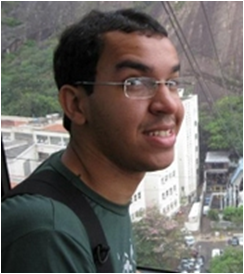
\includegraphics[height=.5\textheight]{images/esdras.png}
		  		\end{center}
			\column{.6 \textwidth}  		
				\begin{block}{Formação}
					\begin{center}
						{\normalsize {\bf Bacharel} em Sistemas de Informação\\
						{\bf Mestre} em Representação Conhecimento (IA)}
					\end{center}
				\end{block}		  		
		  		\begin{block}{Quem?}
		  			\begin{center}
						{\bf Esdras Lins Bispo Junior} \\ Recife, Pernambuco.
					\end{center}
				\end{block}
		\end{columns}
	\end{frame}
	
	\subsection{Informações Importantes}
	\begin{frame}{Informações Importantes}
		\begin{block}{Professor}
			\begin{itemize}
				\item Esdras Lins Bispo Jr.
				\item \url{bispojr@ufg.br}
				\item Sala 18, 1º Andar (Bloco Novo dos Professores)
			\end{itemize}
		\end{block}
	\end{frame}	
	
	\begin{frame}{Informações Importantes}
		\begin{block}{Disciplina}
			\begin{itemize}
				\item Teoria da Computação
				\item 09h30-11h10 (Segunda, [CA2, Sala 05])\\
					  13h30-15h10 (Quinta, [CA2, Sala 11])
				\item Dúvidas: 07h30 - 09h00 (Segunda)\\
					  {\color{red}[é necessário confirmação comigo]}
				\item Grupo: \url{facebook.com/groups/teocomp.ufj.2018.1/}
				\item Repositório: \url{github.com/bispojr/teoria-computacao}
			\end{itemize}
		\end{block}
	\end{frame}
	
	\begin{frame}{Informações Importantes}
		\begin{block}{Metodologia}
			\begin{itemize}
				\item Aulas expositivas utilizando quadro negro (ou branco) e DataShow;
				\item Atendimento individual ou em grupos;
				\item Aplicação de listas de exercícios;
				\item Tempo de Aula: 50 minutos.
			\end{itemize}
		\end{block}
	\end{frame}
	
	\subsection{Instrumentos de Avaliação}
	\begin{frame}{Instrumentos de Avaliação}
		\begin{block}{Mini-Testes}
			\begin{itemize}
				\item MT$_1$ $\Rightarrow$ 20\% da pontuação total;
				\item MT$_2$ $\Rightarrow$ 20\% da pontuação total;
				\item MT$_3$ $\Rightarrow$ 20\% da pontuação total;
				\item MT$_4$ $\Rightarrow$  20\% da pontuação total.
			\end{itemize}
		\end{block} \pause
		\begin{block}{Exercícios-Bônus (EB)}
			Serão propostos EBs, durante toda a disciplina.
		\end{block}
	\end{frame}

	\begin{frame}{Instrumentos de Avaliação}
		\begin{block}{Prova Final (PF) - 20\% da pontuação total}
			A PF é composta por duas etapas: a PF$_1$ e a PF$_2$. 
			A PF$_1$ é composta por dois mini-testes de caráter substitutivo: \pause 
			\begin{itemize}
				\item o SMT$_1$ (referente ao MT$_1$), e 
				\item o SMT$_2$ (referente ao MT$_2$).
			\end{itemize} \pause
			Por sua vez, a PF$_2$ é composta pelos outros dois mini-testes também de caráter substitutivo:  \pause
			\begin{itemize}
				\item o SMT$_3$ (referente ao MT$_3$), e 
				\item o SMT$_4$ (referente ao MT$_4$).
			\end{itemize}
		\end{block}
	\end{frame}

	 \begin{frame}{Informações Importantes}
		\begin{block}{Exercícios-Bônus}
			\begin{itemize}
				\item Semanalmente serão disponibilizados exercícios-bônus (EB) valendo 0,5 ponto na média (quarta-feira, normalmente); \pause
				\item Será dado um prazo para as candidaturas\\
				(normalmente um dia); \pause
				\item Será dada prioridade às candidaturas aos seguintes alunos: \pause
				\begin{enumerate}
					\item Respondeu a nenhum EB; \pause
					\item Respondeu a um EB; \pause
					\item Respondeu a dois EBs; \pause
					\item e assim por diante.
				\end{enumerate} \pause
				\item Haverá sorteio entre candidatos dentro da mesma prioridade; \pause
				\item Uma semana após, o candidato apresentará a sua resposta [texto escrito e slides] (normalmente na quinta, 09h30).
			\end{itemize}
		\end{block}
	\end{frame}
	
	\begin{frame}{Avaliação}
		\begin{block}{Média Final}
			O cálculo da média final será dada da seguinte forma:
			\begin{itemize}
				\item MF = MIN(10, PONT)
			\end{itemize}
			em que MIN representa o mínimo entre dois valores e PONT representa a pontuação total obtida em toda a disciplina, dada da seguinte forma:
			\begin{center}
				PONT = $\left[ \sum\limits_{i=1}^{4} \mbox{max}(MT_i, SMT_i) + PF \right] \times 0,2 + EB$
			\end{center}
		\end{block} \pause
		\begin{exampleblock}{Previsão de Término das Atividades}
			23 de julho de 2018
		\end{exampleblock}
	\end{frame}
	
	\subsection{Distintivos Digitais}
	\begin{frame}{Distintivos Digitais}
		\begin{block}{Como será?}
			Os alunos que estiverem entre as 3 melhores notas de cada avaliação receberão um distintivo digital.
		\end{block} \pause
		\begin{block}{Quantos distintivos existem?}
			\begin{itemize}
				\item {\sc Top One}
				\item {\sc Top Two}
				\item {\sc Top Three}
			\end{itemize}
		\end{block}
	\end{frame}
	
	\begin{frame}{Distintivos Digitais}
		\begin{block}{}
			\begin{center}
				
\includegraphics[height=.65\textheight]{images/badges/top-three.png}
			\end{center}		
			Obter a 3ª melhor nota da turma em uma avaliação. 
		\end{block}
	\end{frame}

	\begin{frame}{Distintivos Digitais}
		\begin{block}{}
			\begin{center}
				
\includegraphics[height=.65\textheight]{images/badges/top-two.png}
			\end{center}		
			Obter a 2ª melhor nota da turma em uma avaliação. 
		\end{block}
	\end{frame}
	
	\begin{frame}{Distintivos Digitais}
		\begin{block}{}
			\begin{center}
				
\includegraphics[height=.65\textheight]{images/badges/top-one.png}
			\end{center}		
			Obter a melhor nota da turma em uma avaliação. 
		\end{block}
	\end{frame}
	
	\begin{frame}{Distintivos Digitais}
		\begin{block}{Pontuação}
			\begin{itemize}
				\item Obter um {\sc Top One}: 10 pontos;
				\item Obter um {\sc Top Two}: 8 pontos;
				\item Obter um {\sc Top Three}: 6 pontos.
			\end{itemize}
		\end{block} \pause
		\begin{exampleblock}{Na Prova Final...}
			Os três primeiros que obtiverem maior pontuação, nos quatro testes, ganharão medalhas.
		\end{exampleblock} \pause
		\begin{block}{Por que estamos usando distintivos digitais?}
			\begin{itemize}
				\item Pode aumentar a motivação dos alunos; \\ \pause
				{\color{blue} (Estou pesquisando para saber se isto é verdade...)}
			\end{itemize}
		\end{block}
	\end{frame}
	
	\begin{frame}{Informações Importantes}
		\begin{block}{Conteúdo do Curso}
			\begin{enumerate}
				\item Introdução à Teoria da Computação;
				\item Modelos de Computação;
				\item Problemas decidíveis;
				\item Problemas indecidíveis;
				\item Complexidade de tempo;
				\item NP-Completude;
				\item Tópicos Avançados.
			\end{enumerate}
		\end{block}
	\end{frame}

%------------------------------------------
	\section{Pensamento}
	\begin{frame}{Pensamento}
  		\begin{center}
    		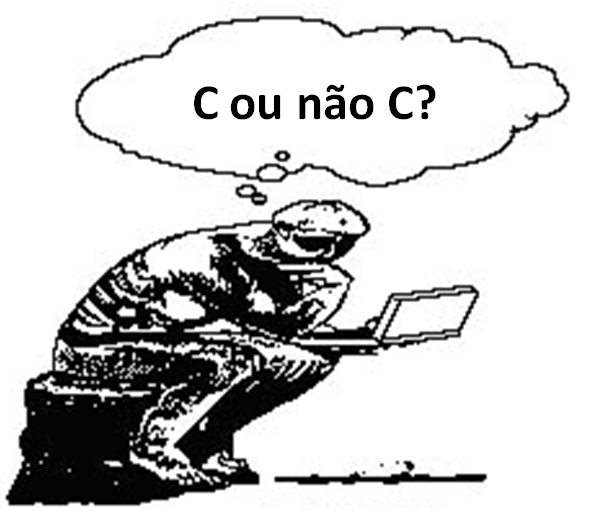
\includegraphics[width=7cm]{images/pensamento.png}
  		\end{center}
	\end{frame}
	
	\begin{frame}{Pensamento}
		\begin{columns}
			\column{.4\textwidth}  		
		  		\begin{center}
		    		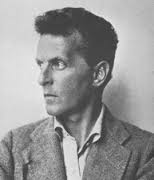
\includegraphics[height=.5\textheight]{images/wittgenstein.jpg}
		  		\end{center}
			\column{.6\textwidth}  		
				\begin{block}{Frase}
					\begin{center}
						{\large Os limites do meu conhecimento são os limites do meu mundo.}
					\end{center}
				\end{block}		  		
		  		\begin{block}{Quem?}
		  			\begin{center}
						{\bf Ludwig Wittgenstein (1889-1951)} \\ Filósofo austríaco.
					\end{center}
				\end{block}
		\end{columns}
	\end{frame}
%------------------------------------------
	\section{Introdução}
	\subsection{O que é Teoria da Computação?}
	\begin{frame}{O que é Teoria da Computação?}
		Pode ser dividida em três grandes áreas:
		\begin{itemize}
			\item Teoria dos Autômatos;
			\item Teoria da Computabilidade;
			\item Teoria da Complexidade.	
		\end{itemize}\pause
		São interligadas pela pergunta:
		\begin{block}{}
			Quais são as capacidades e limitações fundamentais dos computadores?
		\end{block}
	\end{frame}
	
	\begin{frame}{O que é Teoria da Computação?}
		\begin{block}{Teoria dos Autômatos}
			Quais são as definições e propriedades dos modelos matemáticos de computação?
		\end{block} \pause
		\begin{block}{Teoria da Computabilidade}
			O que faz alguns problemas serem solúveis e outros não?		
		\end{block} \pause
		\begin{block}{Teoria da Complexidade}
			O que faz alguns problemas serem computacionalmente difíceis e outros fáceis?
		\end{block}
	\end{frame}
	
	\section{Máquina de Turing}
	\begin{frame}{Modelos Básicos Computacionais}
		\begin{block}{AFDs, AFNs, e Expressões Regulares}
			\begin{itemize}
				\item Potencialidades: reconhecem linguagens como $({\tt 10} \cup {\tt 1})^*$;
				\item Fragilidades: não reconhecem linguagens como $A = \{ {\tt 0}^n {\tt 1}^n \mbox{ | } n \geq 0 \mbox{ e } n \in \mathbb{N} \}$.
			\end{itemize}
		\end{block} \pause
		\begin{block}{GLCs e Autômatos com Pilha}
			\begin{itemize}
				\item Potencialidades: reconhecem linguagens como $A = \{ {\tt 0}^n {\tt 1}^n \mbox{ | } n \geq 0 \mbox{ e } n \in \mathbb{N} \}$;
				\item Fragilidades: não reconhecem linguagens como $A = \{ {\tt a}^n {\tt b}^n {\tt c}^n\mbox{ | } n \geq 0 \mbox{ e } n \in \mathbb{N} \}$.
			\end{itemize}
		\end{block} \pause
		\begin{alertblock}{}
			Portanto são bem restritos para servir de modelo de computadores de propósito geral.
		\end{alertblock}
	\end{frame}
	
	\begin{frame}{Máquinas de Turing (MT)}
		\begin{itemize}
			\item Modelo mais poderoso que GLCs e AFDs; \pause
			\item Turing, 1936; \pause
			\item Características importantes:
				\begin{enumerate}
					\item faz tudo o que um computador real pode fazer;
					\item existem certos problemas que uma MT não pode resolver.
				\end{enumerate}				 
		\end{itemize}
	\end{frame}
	
	\begin{frame}
		\titlepage
	\end{frame}
	
\end{document}